\chapter{Evaluation Results}

\label{AppendixA}

\lhead{Appendix A. \emph{Evaluation Results}}


\section{Clustering results}
\label{eval:sec:clustering_results}

\emph{@TODO: Improve description of data.}

To know what types of users we are dealing with through the next chapters, let's walk through the clusters discovered in the February dataset, as described above.

\begin{figure}
  \centering
  \begin{subfigure}[t]{0.45\textwidth}
    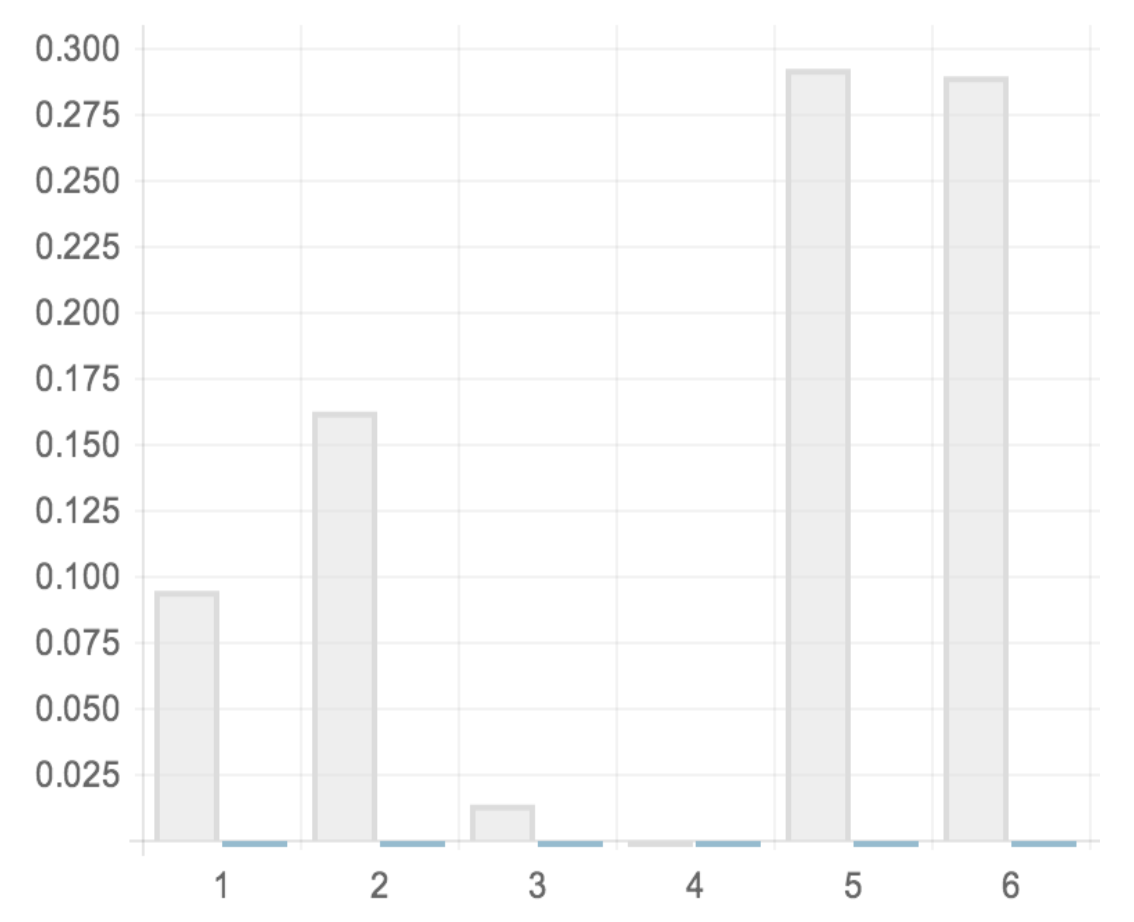
\includegraphics[width=\textwidth]{Figures/clusterings/confluence-post/cluster1-chart}
    \caption{Cluster 1: Front page hitting users}
    \label{fig:cluster1-chart}
  \end{subfigure}
  \hfill
  \begin{subfigure}[t]{0.45\textwidth}
    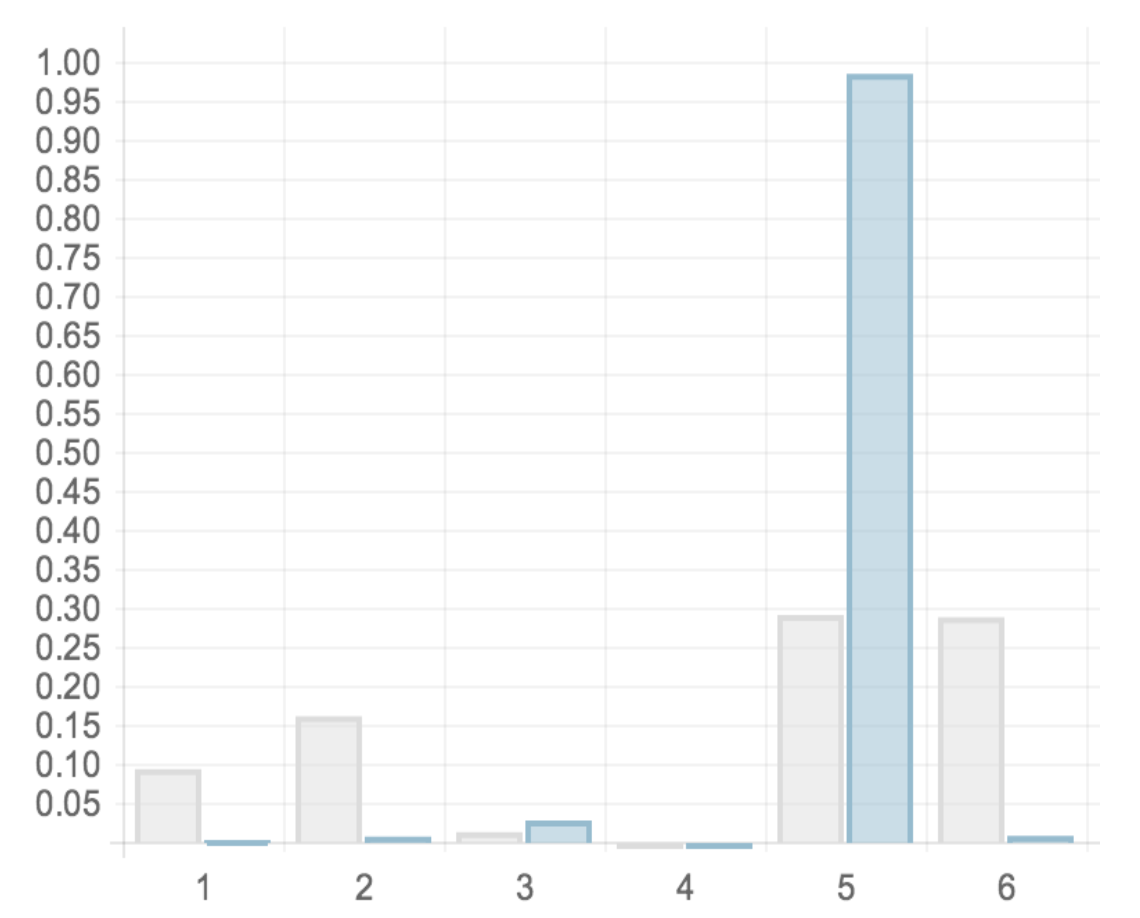
\includegraphics[width=\textwidth]{Figures/clusterings/confluence-post/cluster2-chart}
    \caption{Cluster 2: Users trying out the service alone}
    \label{fig:cluster2-chart}
  \end{subfigure}

  \begin{subfigure}[t]{0.45\textwidth}
    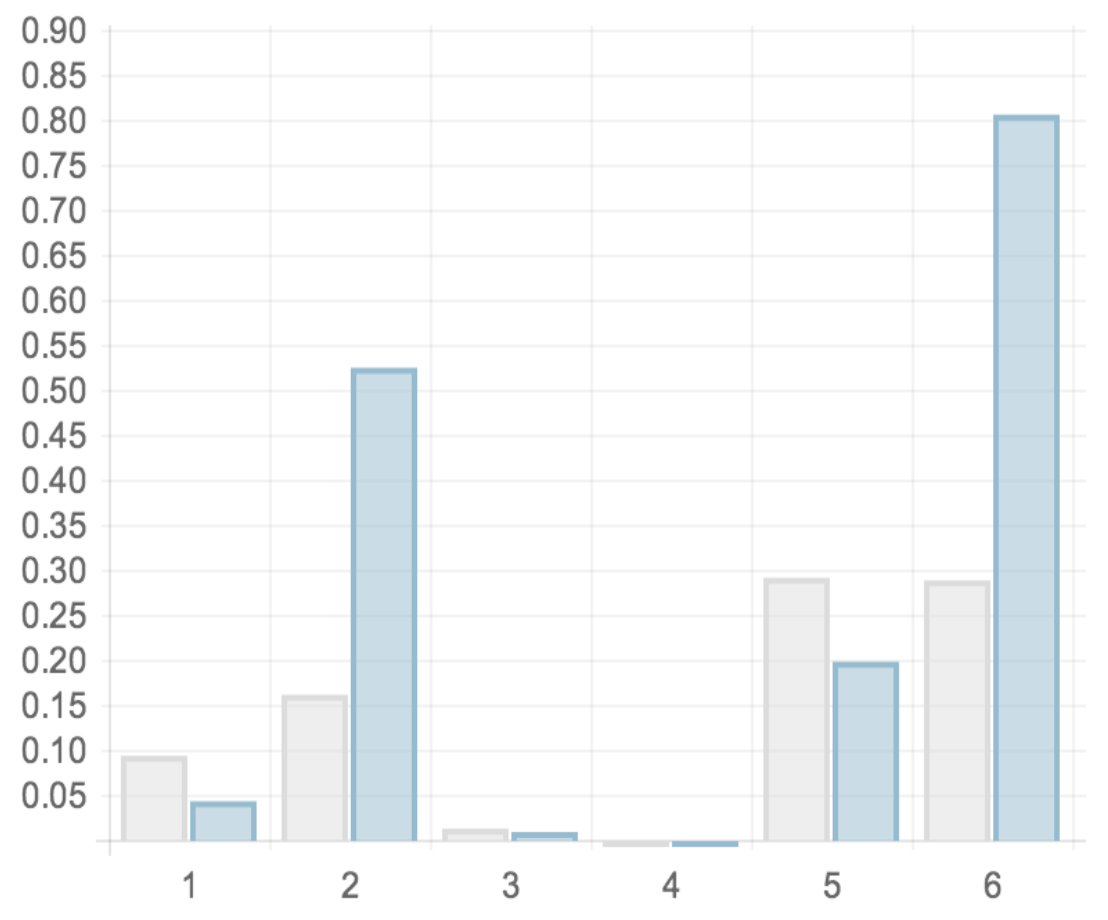
\includegraphics[width=\textwidth]{Figures/clusterings/confluence-post/cluster3-chart}
    \caption{Cluster 3: Simple users with small networks}
    \label{fig:cluster3-chart}
  \end{subfigure}
  \hfill
  \begin{subfigure}[t]{0.45\textwidth}
    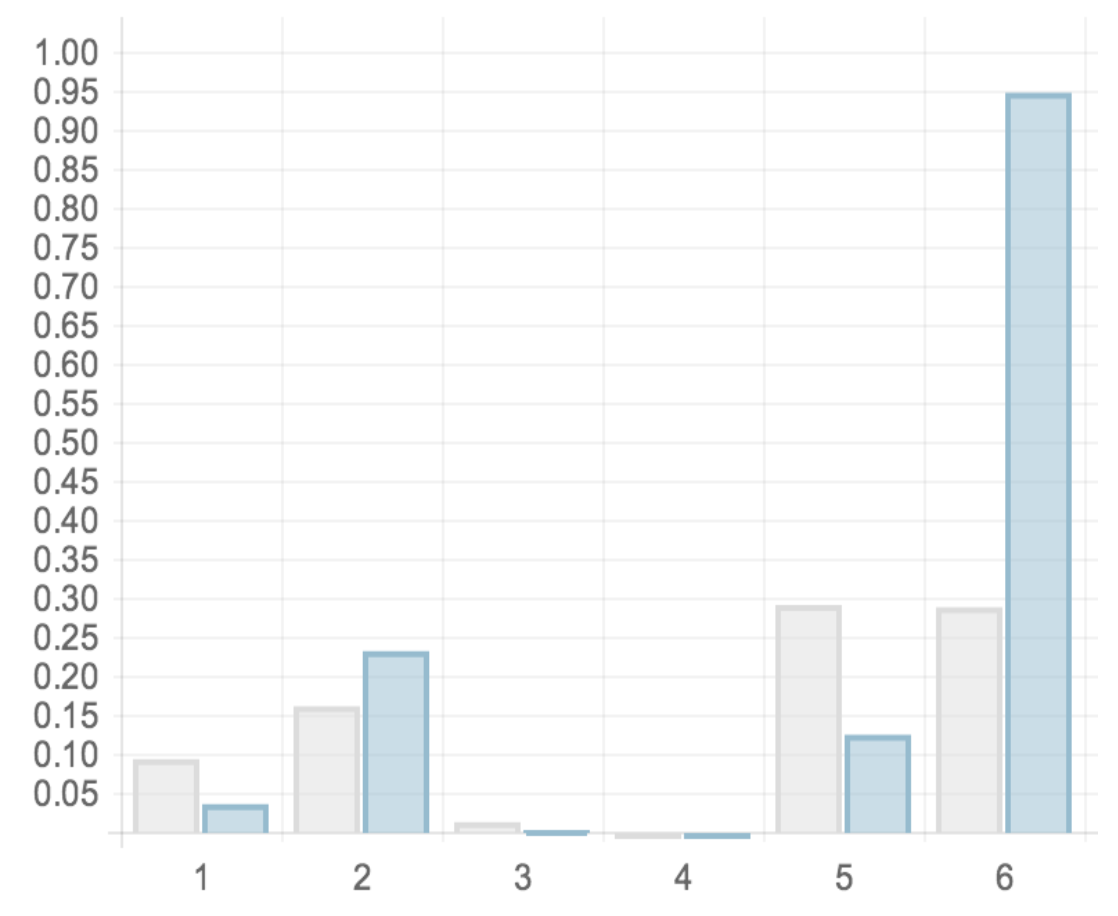
\includegraphics[width=\textwidth]{Figures/clusterings/confluence-post/cluster4-chart}
    \caption{Cluster 4: Simple users with large networks}
    \label{fig:cluster4-chart}
  \end{subfigure}

  \begin{subfigure}[t]{0.45\textwidth}
    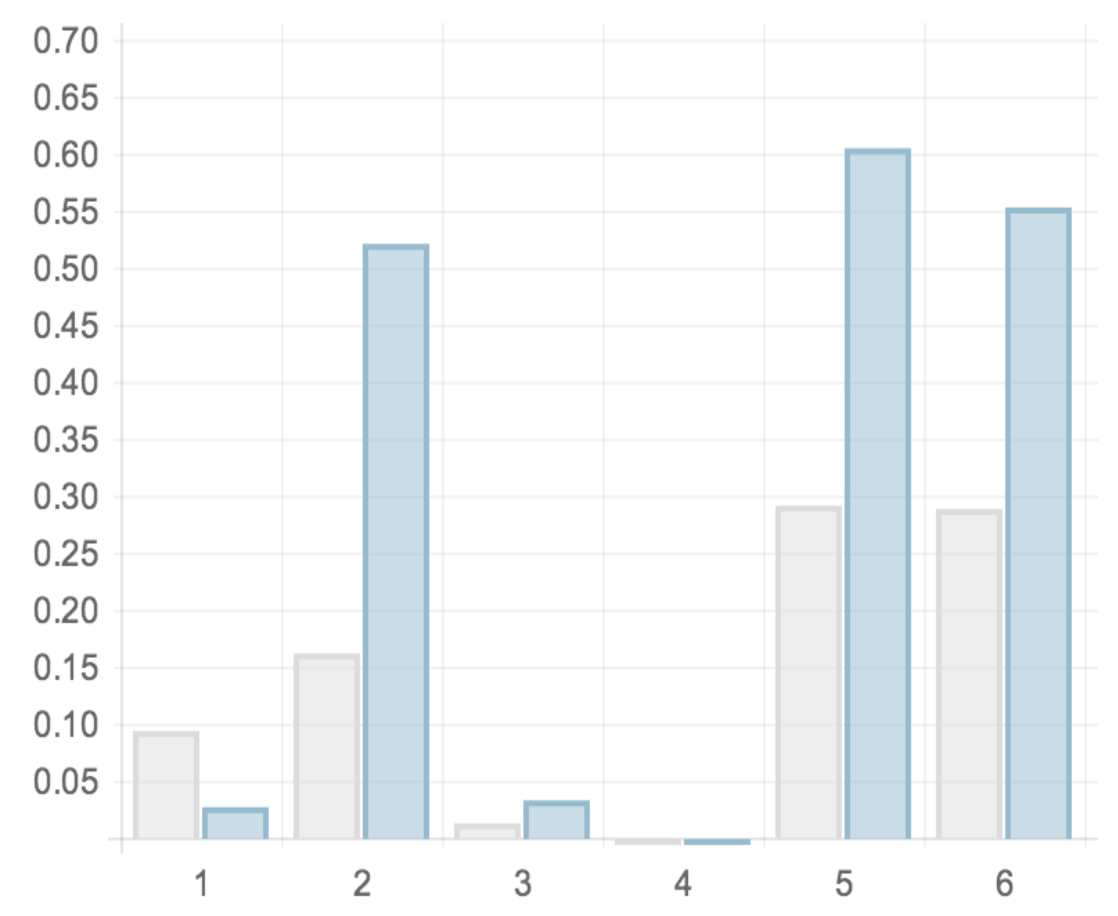
\includegraphics[width=\textwidth]{Figures/clusterings/confluence-post/cluster5-chart}
    \caption{Cluster 5: Incognito users}
    \label{fig:cluster5-chart}
  \end{subfigure}
  \hfill
  \begin{subfigure}[t]{0.45\textwidth}
    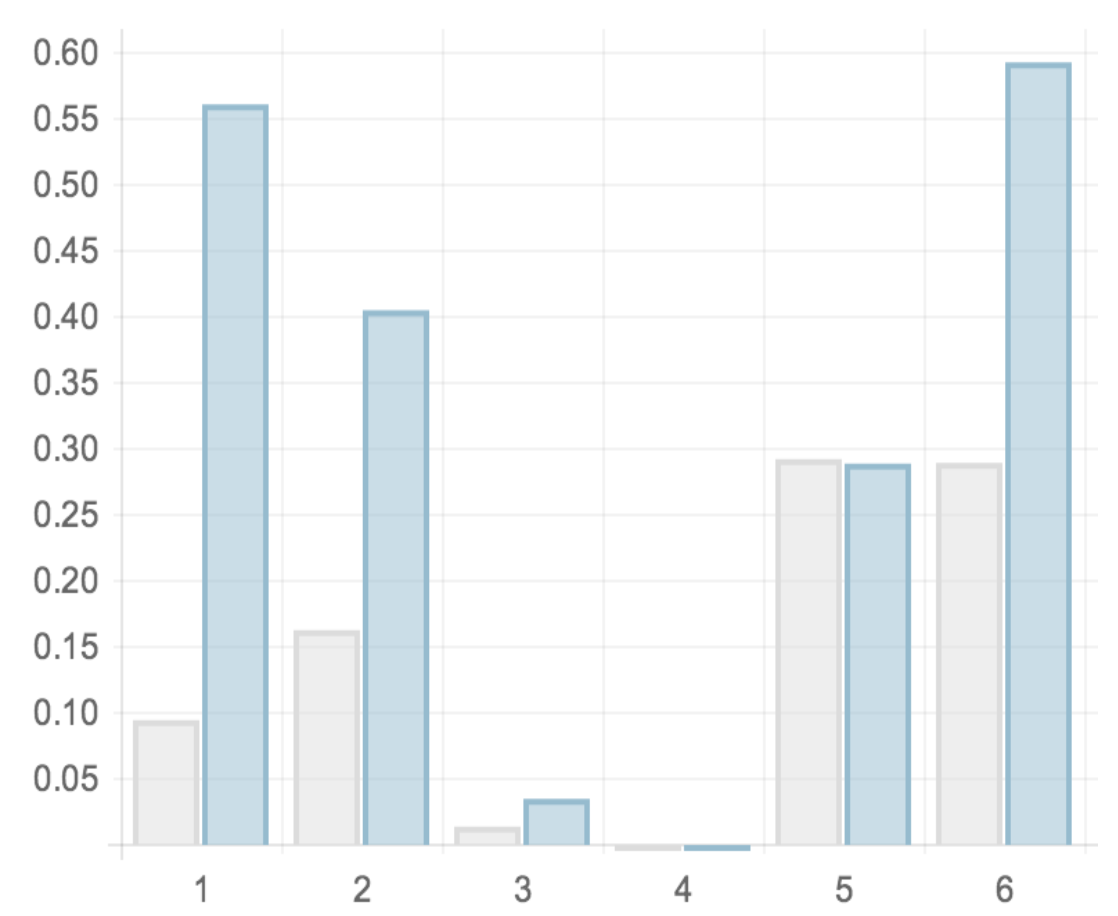
\includegraphics[width=\textwidth]{Figures/clusterings/confluence-post/cluster6-chart}
    \caption{Cluster 6: Chatty, simple users}
    \label{fig:cluster6-chart}
  \end{subfigure}

  \caption{Cluster centers compared to the unweighted average cluster centers. \\ The features plotted are 1) chat messages sent, 2) conversations, 3) rooms claimed, 4) rooms followed, 5) unique rooms used, and 6) conversation network size.}
\end{figure}

\subsection{Cluster 1: Front page hits}

The centroid for this cluster is quite simply $\mu_1 = \langle 0, 0, 0, 0, 0, 0 \rangle$.

\begin{persona}
  The user has not tried the actual service -- most likely hitting the front page and either not using a compatible device/browser, or not finding it interesting enough to try out.
\end{persona}

\subsection{Cluster 2: Trying out the service alone}

As shown in figure~\ref{fig:cluster2-chart}, the users in this cluster score close to 0 on every feature except the number of rooms used -- most notably, the number of conversations.

\begin{persona}
  The user has tried out the service, but not ever conversed with another user.
\end{persona}

\subsection{Cluster 3: Simple users with small networks}

Users in cluster 3 (see figure~\ref{fig:cluster3-chart}) don't use any of the more advanced features of the service, like chatting, claiming or following a room, but on average they have taken part in just over 5 conversations.

\begin{persona}
  A returning user, only utilizing the bare functionality, conversing only with a very limited group of people.
\end{persona}

\subsection{Cluster 4: Simple users with large networks}

The users in cluster 4 (see figure~\ref{fig:cluster4-chart}) are very much like the ones in cluster 3, but use the service slightly more, and are part of much larger networks.

\begin{persona}
  A returning user, only utilizing the bare functionality, part of a large group of people using the service.
\end{persona}

\subsection{Cluster 5: Incognito users}

To track users over time, cookies are required. Whenever clearing the browser cache, or when browsing in ``incognito mode''\footnote{Browsing without storing any data, including cookies.}, the service will not be able to tie together user sessions. These perceived one-off users should end up in this cluster, close to the pattern shown in figure~\ref{fig:cluster5-chart}.

\begin{persona}
  A user browsing in incognito mode, or who clears the browser cache regularly.
\end{persona}

\subsection{Cluster 6: Chatty simple users}

The users of cluster 6 are very much like those in cluster 3, as can be seen in figure~\ref{fig:cluster6-chart}. The significant difference is that they make heavy use of the chat functionality.

\begin{persona}
  A user sharing the characteristics of users in cluster 3, except in making use of the text chat functionality.
\end{persona}
